
%*****************************************
\chapter{Developing the concept FiPa}\label{ch:forth}
%*****************************************
The following chapter represents a concept called \underline{\textbf{FiPa}} (\underline{\textbf{Fi}}nd \underline{\textbf{Pa}}ttern) which was developed to contribute towards the ongoing work of Zezschwitz et al. \cite{Zezschwitz}, discussed in Chapter \ref{ch:third}. Before entering into the development process, it is crucial to note that the following concept was created solely to serve as a tool in the user case study, which will be presented in Chapter \ref{ch:fifth}. The system is in no means a suggestion for an authentication concept and was not intended to be utilized as such. Its sole purpose was meant for the scope of this thesis, and no further. Therefore certain aspects (e.g., security and effectiveness) have consciously not been considered during the design and the development of this concept. Nonetheless, the design process was based on a  \textbf{User-Centered Design} (UCD) approach and included a selection of \textbf{Human Computer Interaction} (HCI) principles, to make the concept easier to understand and function. The exact procedure of this process will be documented through the direct voice of the author to convey her thought process and intentions in this part of her contribution towards this thesis. 

\section{Requirements} \label{4.1}
As mentioned above, the concept was intended to be utilized as a tool to help examine certain factors later on in the study, which are \textit{orientation time} and \textit{input time}, previously introduced in Chapter \ref{ch:third}. In order to do so, the nature of the concept had to be specially designed to suit the anatomy of an authentication process. The concept had to be divided into two coherent and related small tasks: a \textbf{mental task} and a \textbf{practical task}. The intention behind this division was to be able to measure the \textit{orientation time} (duration of the mental task) and the \textit{input time} (duration of the practical task), separately. For that, a timer feature had to be implemented, in order to undertake the measurements, which would automatically be saved in a local database (see Section \ref{4.3}).\\

Furthermore, as indicated in Section \ref{3.3}, the goal of the research contribution in this thesis, is to examine the impact that \textit{orientation time} has on the perceived efficiency of an authentication concept, with respect to its \textit{input time}. To complement and also validate the findings from the ongoing study by Zezschwitz et al. \cite{Zezschwitz}, we proposed to analyze the following two contrasting time ratios:  
\begin{center}
    "\textcolor{blue}{long} orientation/\textcolor{red}{short} input" \\
    \textbf{vs.} \\
    "\textcolor{red}{short} orientation/\textcolor{blue}{long} input".
\end{center} 

The crossing descriptors \textit{long} and \textit{short} were meant to define a certain length, meaning \textit{long orientation} had to have the same duration as \textit{long input}, and vice versa. In order to have a baseline to which the measured times of the ratios above could be compared, a third ratio was included. It is called \textcolor{red}{short} orientation/\textcolor{red}{short} and its \textit{orientation time} and \textit{input time} are equally long. \\
 

In addition, we were interested in directly comparing both contrasting ratios against each other by using \textit{only one concept}, instead of three (see Chapter \ref{ch:third}). Through unifying all three ratios into one concept, it was possible to eliminate the chance of future results being influenced by the study participants' personal preferences of the concepts.
For that reason, the created concept had to be malleable in a such way, that the complexity of each task (\textbf{mental} and \textbf{practical}) could be adjusted, according to the represented ratio. For "long phases", we intended to be represented through difficult tasks (\textbf{mental} or \textbf{practical}). An analogous approach was taken for the "short phases" of the ratios.

\begin{figure}[t!]
\centering
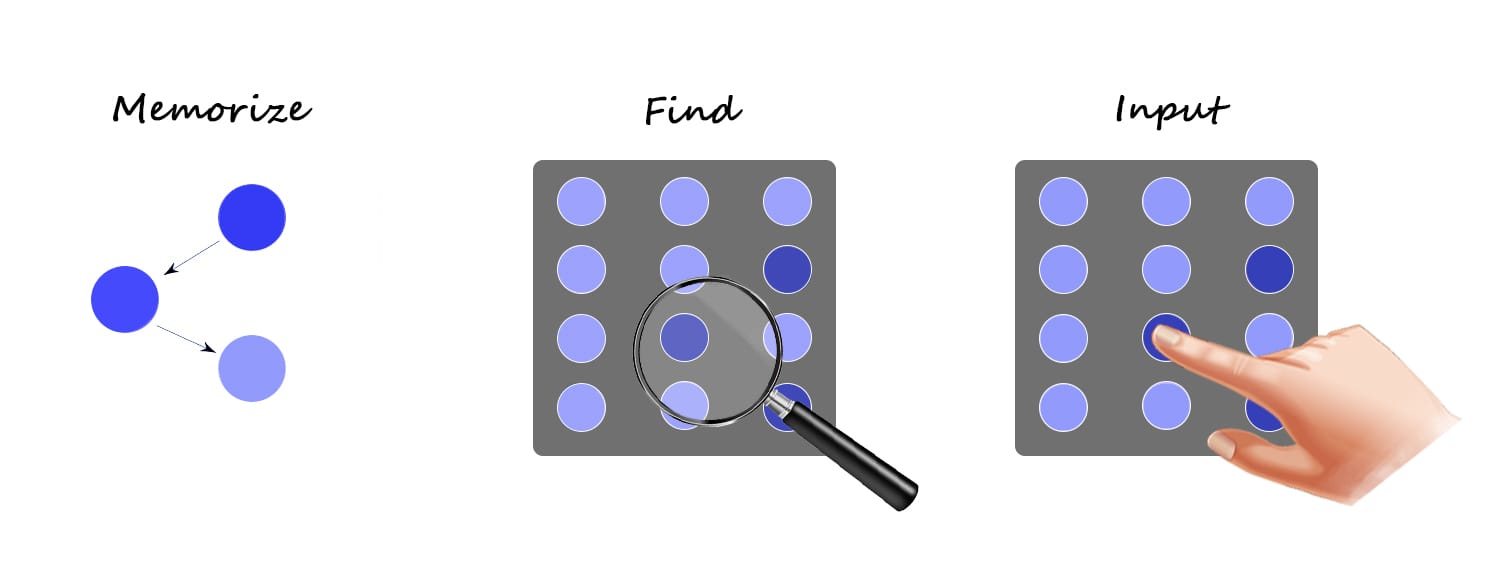
\includegraphics[width=15cm, height=6cm]{Chapters/graphics/ConceptIdea.jpeg}
\caption{Simple illustration of the initial idea for \underline{\textbf{FiPa}}. The procedure is composed of three steps: (1) \textbf{Memorize} a pattern; (2) \textbf{Find} the memorized pattern, hidden inside a grid; (3) \textbf{Input} of the pattern.}
\label{fig:concept}
\end{figure}

\section{Development} \label{4.2}

In the following section, we will present the design and evaluation attempts that were necessary to generate \underline{\textbf{FiPa}}: the concept presented and utilized in our study. 

\subsection{Fundamental Concept Idea} \label{4.2.1}

During the creation of \underline{\textbf{FiPa}}, we were interested in creating a concept which activated an interaction that reminded users of a smartphone authentication. We assumed that by making the interaction resemble an authentication process, future study participants' could better understand and adapt to the context of the study. A further one of our intentions was to construct a concept that was as usable, to direct participants focus and attention towards the actual usability issues, intended for them to test. For that, we decided to create a \textit{graphic-based concept}, as researchers have discovered them to be commonly accepted by users and perceived as comfortable to use \cite{PatternWild}. \\ 

The name of our concept, \underline{\textbf{FiPa}}, is inspired by its functionality. \underline{\textbf{FiPa}} is an abbreviation for the phrase "\underline{\textbf{Fi}}nd \underline{\textbf{Pa}}ttern" and its meaning will be comprehensible through the following description of its procedure (see Figure \ref{fig:concept}): First, a predefined pattern is presented which has to be memorized well by the user. This pattern consists of a certain combination of buttons. Each button has a certain characteristic, that makes it distinguishable from the others. Memorizing the order of the buttons and their distinct characteristics is crucial for successfully accomplishing the \textbf{mental} and \textbf{practical task} (Section \ref{4.2.1}). After \underline{memorizing} the pattern, a large grid, filled with buttons, is presented. The \textbf{mental task} defined by \underline{finding} the memorized pattern, hidden inside the grid. When found, the \textbf{practical task} is comprised of entering  (\underline{input}) the found pattern correctly into the grid (see Figure \ref{fig:concept}).\\

The idea of using a grid of buttons for the \textbf{mental task} was derived from the concept \textit{Pattern Rotation} \cite{Marbles, Zezschwitz}. The choice of using specific characteristics for each button was inspired by the concept \textit{Marbles} \cite{Marbles, Zezschwitz}\footnote{To familiarize with the concepts \textit{Marbles} and \textit{Pattern Rotation}, please revisit Section \ref{2.2.3} and Chapter \ref{ch:third}.}. We tried to limit the amount of mental effort required for interacting with \underline{\textbf{FiPa}} was reduced as much as possible by making a set of intentional design choices. We assumed the pattern would certainly not be memorized permanently and that it would, therefore, be stored in participants' short-term memory. Therefore, we attempted to reduce the load of mental effort by letting the pattern be searched for, instead of completely reproduced from memory. That way, during the \textbf{mental task}, when the user stumbles upon the hidden pattern inside the grid, they are more likely to detect it because they recognize it. As mentioned above, this is a measure that was taken to ease the interaction with \underline{\textbf{FiPa}} and to shift participants' focus onto the important matters, namely the ratios represented in the study.

\begin{figure}[t!]
\centering
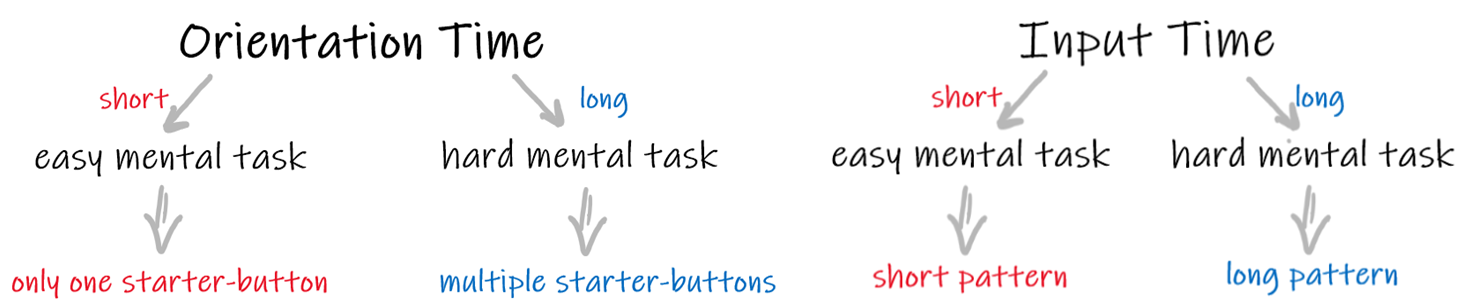
\includegraphics[width=12cm, height=4cm]{Chapters/graphics/OriInput.PNG}
\caption{Depiction of how the \textbf{mental} and \textbf{practical tasks} were intended to be designed, depending on whether \textit{orientation time} and \textit{input time} were long or short.}
\label{fig:orientation_input}
\end{figure}

\subsection{Concept Design} \label{4.2.2}

In the following section the design approaches, that were involved in creating and developing the concept \underline{\textbf{FiPa}}, will be presented.

\begin{figure}[t!]
\centering
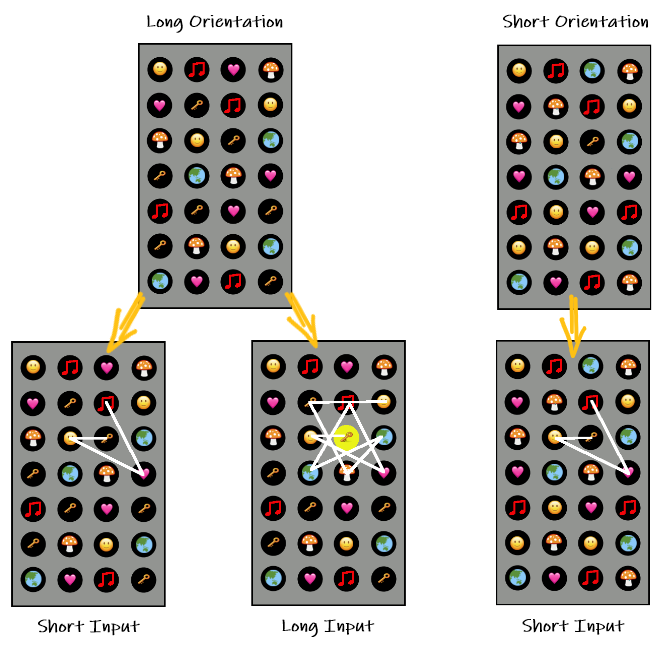
\includegraphics[width=14cm, height=14cm]{Chapters/graphics/firstdraft.PNG}
\caption{Detailed representation of the initial layout design for \underline{\textbf{FiPa}}. \textbf{Mental} and \textbf{practical task} are marked to provide a better understanding of the concept.}
\label{fig:firstdraft}
\end{figure}

\subsubsection{First Draft} \label{4.2.2.1}
The initial layout design for \underline{\textbf{FiPa}} is illustrated in figure \ref{fig:firstdraft}. As in \textit{Marbles} \cite{Marbles, Zezschwitz}, different elements of the concept, meaning the buttons, were distinguishable through small images, emojis to be exact. To provide a clear overview of the vision, I will first begin by explaining how we the design for the \textbf{practical task} and then presenting my intentions regarding the \textbf{mental task}. As mentioned in Section \ref{4.1}, the first step of the concept is to memorize a pattern at the very beginning of the activity. For simplicity reasons I decided to mark the beginning of each pattern, by setting their first button to contain a key-emoji (see Figure \ref{fig:firstdraft}). We will call this button the \textit{starter-button}. Examples for the patterns are shown in figure \ref{fig:firstdraft}. Moreover, I envisioned the input method of \underline{\textbf{FiPa}} to be similar to \textit{Android Pattern Unlock}. As the concept is intended to be implemented as smartphone application, I assumed that the chosen method of input would be suitable for a touch screen user interface. \\

For the \textbf{mental task} (see Figure \ref{fig:firstdraft}), the design of the grid depended on whether long \textit{orientation time} or short \textit{orientation time} was intended. As mentioned earlier in Section \ref{4.1}, we assumed that for a long \textit{orientation time}, we need to create a difficult and more complex search process. We imagined that by incorporating multiple \textit{starter-buttons} inside the grid, besides the one belonging to the hidden pattern, we could complicate and elongate the search process. In contrast, we imagined it would be possible to facilitate the pattern search, by having the only \textit{starter-button} in the grid belong to the hidden pattern. That way, our future participants could spot the pattern much easier and quicker. An analogous approach was considered for adjusting the complexity of the \textbf{practical task}. Depending on whether long or short \textit{input time} was intended, the pattern designed for memorization and input was accordingly short or long (see Figure \ref{fig:orientation_input}).

\subsubsection{Evaluation: First Draft} \label{4.2.2.2}

The first draft of \underline{\textbf{FiPa}} was evaluated, using a paper prototype. The prototype encompassed the three ratios (see Section \ref{4.1}) and was composed of three patterns\footnote{Two short patterns intended for \textit{short input time} and one long pattern intended for \textit{long input time}.} and three grids\footnote{Two grids with only one \textit{starter-button}, for \textit{short orientation time} and one grid with multiple \textit{starter-buttons}, for \textit{long orientation time}.}. We used the same grid and pattern constellation, shown in figure \ref{fig:firstdraft}.\\
It was important to examine how the design choices affected the usability of the concept and to see whether it was easy to use and to understand. Six participants were recruited to evaluate the first draft. Before presenting the prototype to each participant, I explained the purpose of the study and the functionality of the prototype. The structure of the prototype was based the concept of \textit{Wizard Of Oz} prototyping \cite{Butz2014}. This meant that during a participant's interaction with the prototype, I would uncover its  following event (grid or pattern), depending on the participant's \textit{input} or \textit{action}.\\

Five of the participants found that the many different emojis created an overwhelming appeal on the eyes and that it made the grid appear very crowded. Moreover, the long pattern (see Figure \ref{fig:firstdraft}) was considered too complicated and was hard to memorize by all of the participants. As mentioned earlier, the reason behind the complicated pattern, was to represent long \textit{input time}. Thus the modified complexity of the pattern was not well accepted, a different solution is called for, to help control the length of the represented \textit{input time}. Nonetheless, the idea behind the concept was liked by all of the participants. Especially, the notion of starting each pattern with a specific \textit{starter-button}. Despite the flaws mentioned above, they understood the basic functioning of our concept well. \\

The information gained and the lessons learned through the previous evaluation phase gave us a closer insight into humans' perception and cognitive ability. At this point, we were one step closer to creating a more usable and effective concept.

\begin{figure}[t!]
\centering
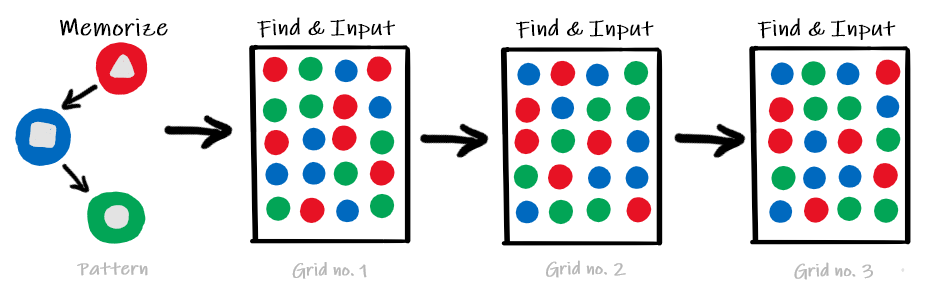
\includegraphics[width=13cm, height=5cm]{Chapters/graphics/seconddraft.PNG}
\caption{A sketch that presents the basic structure of each phase of the prototype. Each grid represents a \textbf{couple}: a \textbf{mental task} (find) and a \textbf{practical task} (input). After memorizing the given pattern, three uniquely designed grids followed. The pattern had to be found and entered in each of the grids, one after the other.}
\label{fig:secondDraft}
\end{figure}

\subsubsection{Second Draft} \label{4.2.2.3}

For the second draft of \underline{\textbf{FiPa}}, a few adjustments were made  regarding its overall aesthetics and the design. Through further research, I discovered that due to the \textit{pictorial superiority effect} \cite{pictorial}, humans can retain information through images, much better than through letters or numbers \cite{pictorial, 2014}, which is why I decided to continue representing the characteristics of the buttons through images.\\
To reduce the crowded appeal from the first draft, I replaced the emojis with three simple shapes: \textit{circle}, \textit{square}, and \textit{triangle}. The initial choice of colors for the design was: \textit{red}, \textit{green} and \textit{blue}. They are known to be the basic colors that the human eye perceives naturally \cite{Butz2014}. The \textit{starter-button} was designed to be a red containing a triangle (see Figure \ref{fig:secondDraft}). The triangle shape was chosen because it is a symbol that has been shown to convey the meaning of \textit{power}\footnote{http://www.whiteriverdesign.com/meaning-shapes-design/ - last accessed: 2019/11/16} and \textit{permanence} \cite{Frutiger1998}.  Moreover, the human eye is naturally attracted to its shape \footnote{https://designshack.net/articles/layouts/the-sometimes-hidden-meaning-of-shapes/ - last accessed: 2019/11/16}. I assumed that through the mentioned effect of the triangle and the alerting appeal of the color red, users' vision would initially be attracted to these button through the ability of their \textit{pre-attentive perception} \cite{Butz2014}. \\

To properly design the patterns and grids design of this draft, it was crucial to define a fixed size for the grid. After a few of trials, I found the size 4x7 to be most suitable for the concept, big enough to hold a decent amount of buttons and to provide a clear overview of the grid's content. An additional design feature for this draft are so-called \textit{traps}. \textit{Traps} are a set of buttons, that have a similar constellation and set of characteristics as the hidden pattern, yet are not identical to it. Their purpose is to mislead the user, during the \textbf{mental task} and thereby elongate the search process as needed. Another modification made was the input method. As participants did not improve of the complexity of the long pattern, in the first draft, I decided to change the input method. I discovered that pressing the buttons in the right order, instead of connecting them (see Section \ref{4.2.2.1}), would allow more control over the approximate duration of the \textit{input time}. That way, long \textit{input time} could represented without requiring participants to memorize complicated patterns. Moreover, the created patterns no longer covered much space inside the grid, which made it easier to shuffle the buttons and set more \textit{traps}. 

\begin{figure}[t!]
\centering
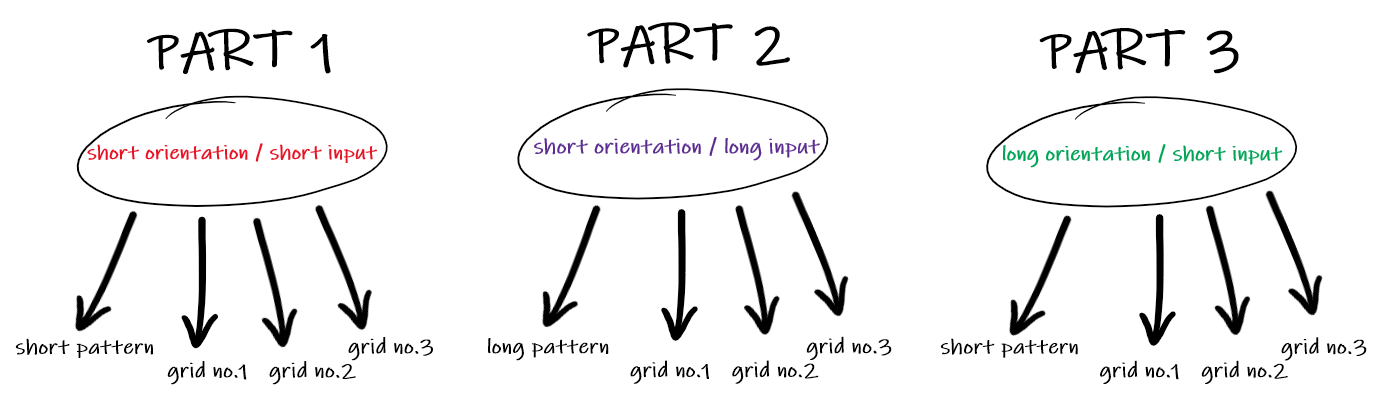
\includegraphics[width=13cm, height=5cm]{Chapters/graphics/prototypeStructure.PNG}
\caption{Simple representation of the structure of the second design. Each part is assigned to a particular ratio. For each ratio there are three grids. Each grid presents a \textbf{mental task} (find) and \textbf{practical task} (input), a so called \textbf{couple}. The order of the ratios presented in this figure is only a suggestion. The exact order of the ratios was not important in the evaluation phase.}
\label{fig:prototype}
\end{figure}

\subsubsection{Evaluation: Second Draft} \label{4.2.2.4}

Analogous to the evaluation of the first draft (see Section \ref{4.2.2.2}), I created a \textit{Wizard of Oz} \cite{Butz2014} paper prototype (see Figure \ref{fig:paperprototype}) to evaluate the changes and improvements, made in the second draft of the concept. However, this time, the prototype was created differently. I was interested in testing a certain structure for the concept to see if it would be suitable for the its implementation as a smartphone application. The paper prototype was structured into \underline{three parts} as there are three ratios (see Section \ref{4.1}) to examine. In the previous draft, there was only one \textbf{mental} and \textbf{practical task} per ratio. For simplicity, we will call the pairing of a  \textbf{mental} and a \textbf{practical task}, a \textbf{couple}. Instead of having only one \textbf{couple} per ratio (as in the first draft), I decided to assign three couples to each ratio (see Figure \ref{fig:prototype}). My intention behind this decision was to assure that participants would have a better memory of the different ratios during the qualitative segment of the study, if they interacted with each one more than once. The modification of the concept was tested with the same set of participants who tested the first draft, in order to receive a more detailed feedback on whether the flaws, detected in the previous draft, were correctly fixed. It was possible to interview the same set of participants, as the design and the structure of the \textbf{mental} and \textbf{practical tasks} differed completely from the first draft. Fortunately, both, layout and structure of our prototype were well accepted. \\

To ensure that the average duration needed for the accomplishment of the \textbf{mental} and \textbf{practical tasks} corresponded with the represented ratio, I manually timed each participant using a stopwatch. Although each part of the paper prototype was comprised of three \textbf{couples}, only the time measurements for every third \textbf{couple} were. The first and second \textbf{couples} of each part were considered exercises for the participants to get acquainted with the concept. \\
Analogous to the measurement approach made by Zezschwitz et al. \cite{Zezschwitz} (see Chapter \ref{ch:third}), I defined a distinct interval for each of the tasks. A \textbf{mental task} began immediately after a particular grid was uncovered and ended as soon as the hidden pattern was found. A participant would indicate that they found a pattern by tapping its \textit{starter-button}. The \textbf{practical task} began with the \textit{first button press} of a pattern and ended with its the \textit{last button press}. During the input, the \textit{starter-button} had to pressed once again, even if it had already been tapped to signify the find. I was aware that the measured times would not be completely accurate. They were only intended to serve as a rough estimate for the duration of the phases. Fortunately, the designed grids and patterns created for the paper prototype (see Figure) delivered proper time estimates for the represented ratios and were, therefore, suitable to be included in the implementation of the concept.\\

\begin{figure}[t!]
\centering
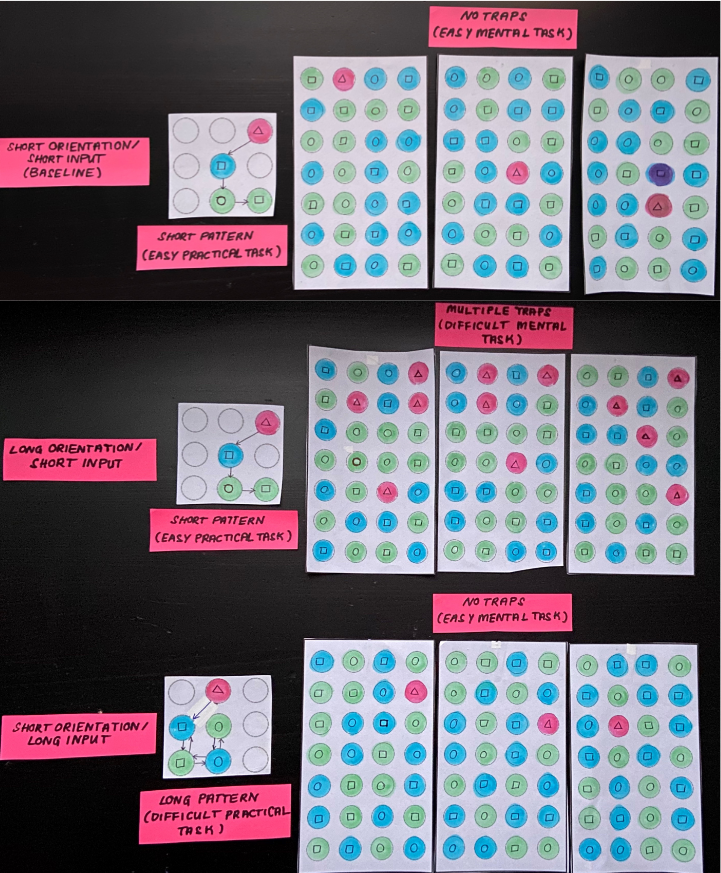
\includegraphics[width=15cm, height=20cm]{Chapters/graphics/paperprototype.PNG}
\caption{This is an picture of the paper prototype which was used to evaluate the second draft of the concept. In the picture the cards are categorized by ratio. To better understand the purpose of the \textit{traps} (see Section \ref{4.2.2.3}), it would be useful to try and search for the pattern, in the three grids of the ratio \textit{long orientation/short input} (middle row).}
\label{fig:paperprototype}
\end{figure}

\begin{figure}[t!]
\centering
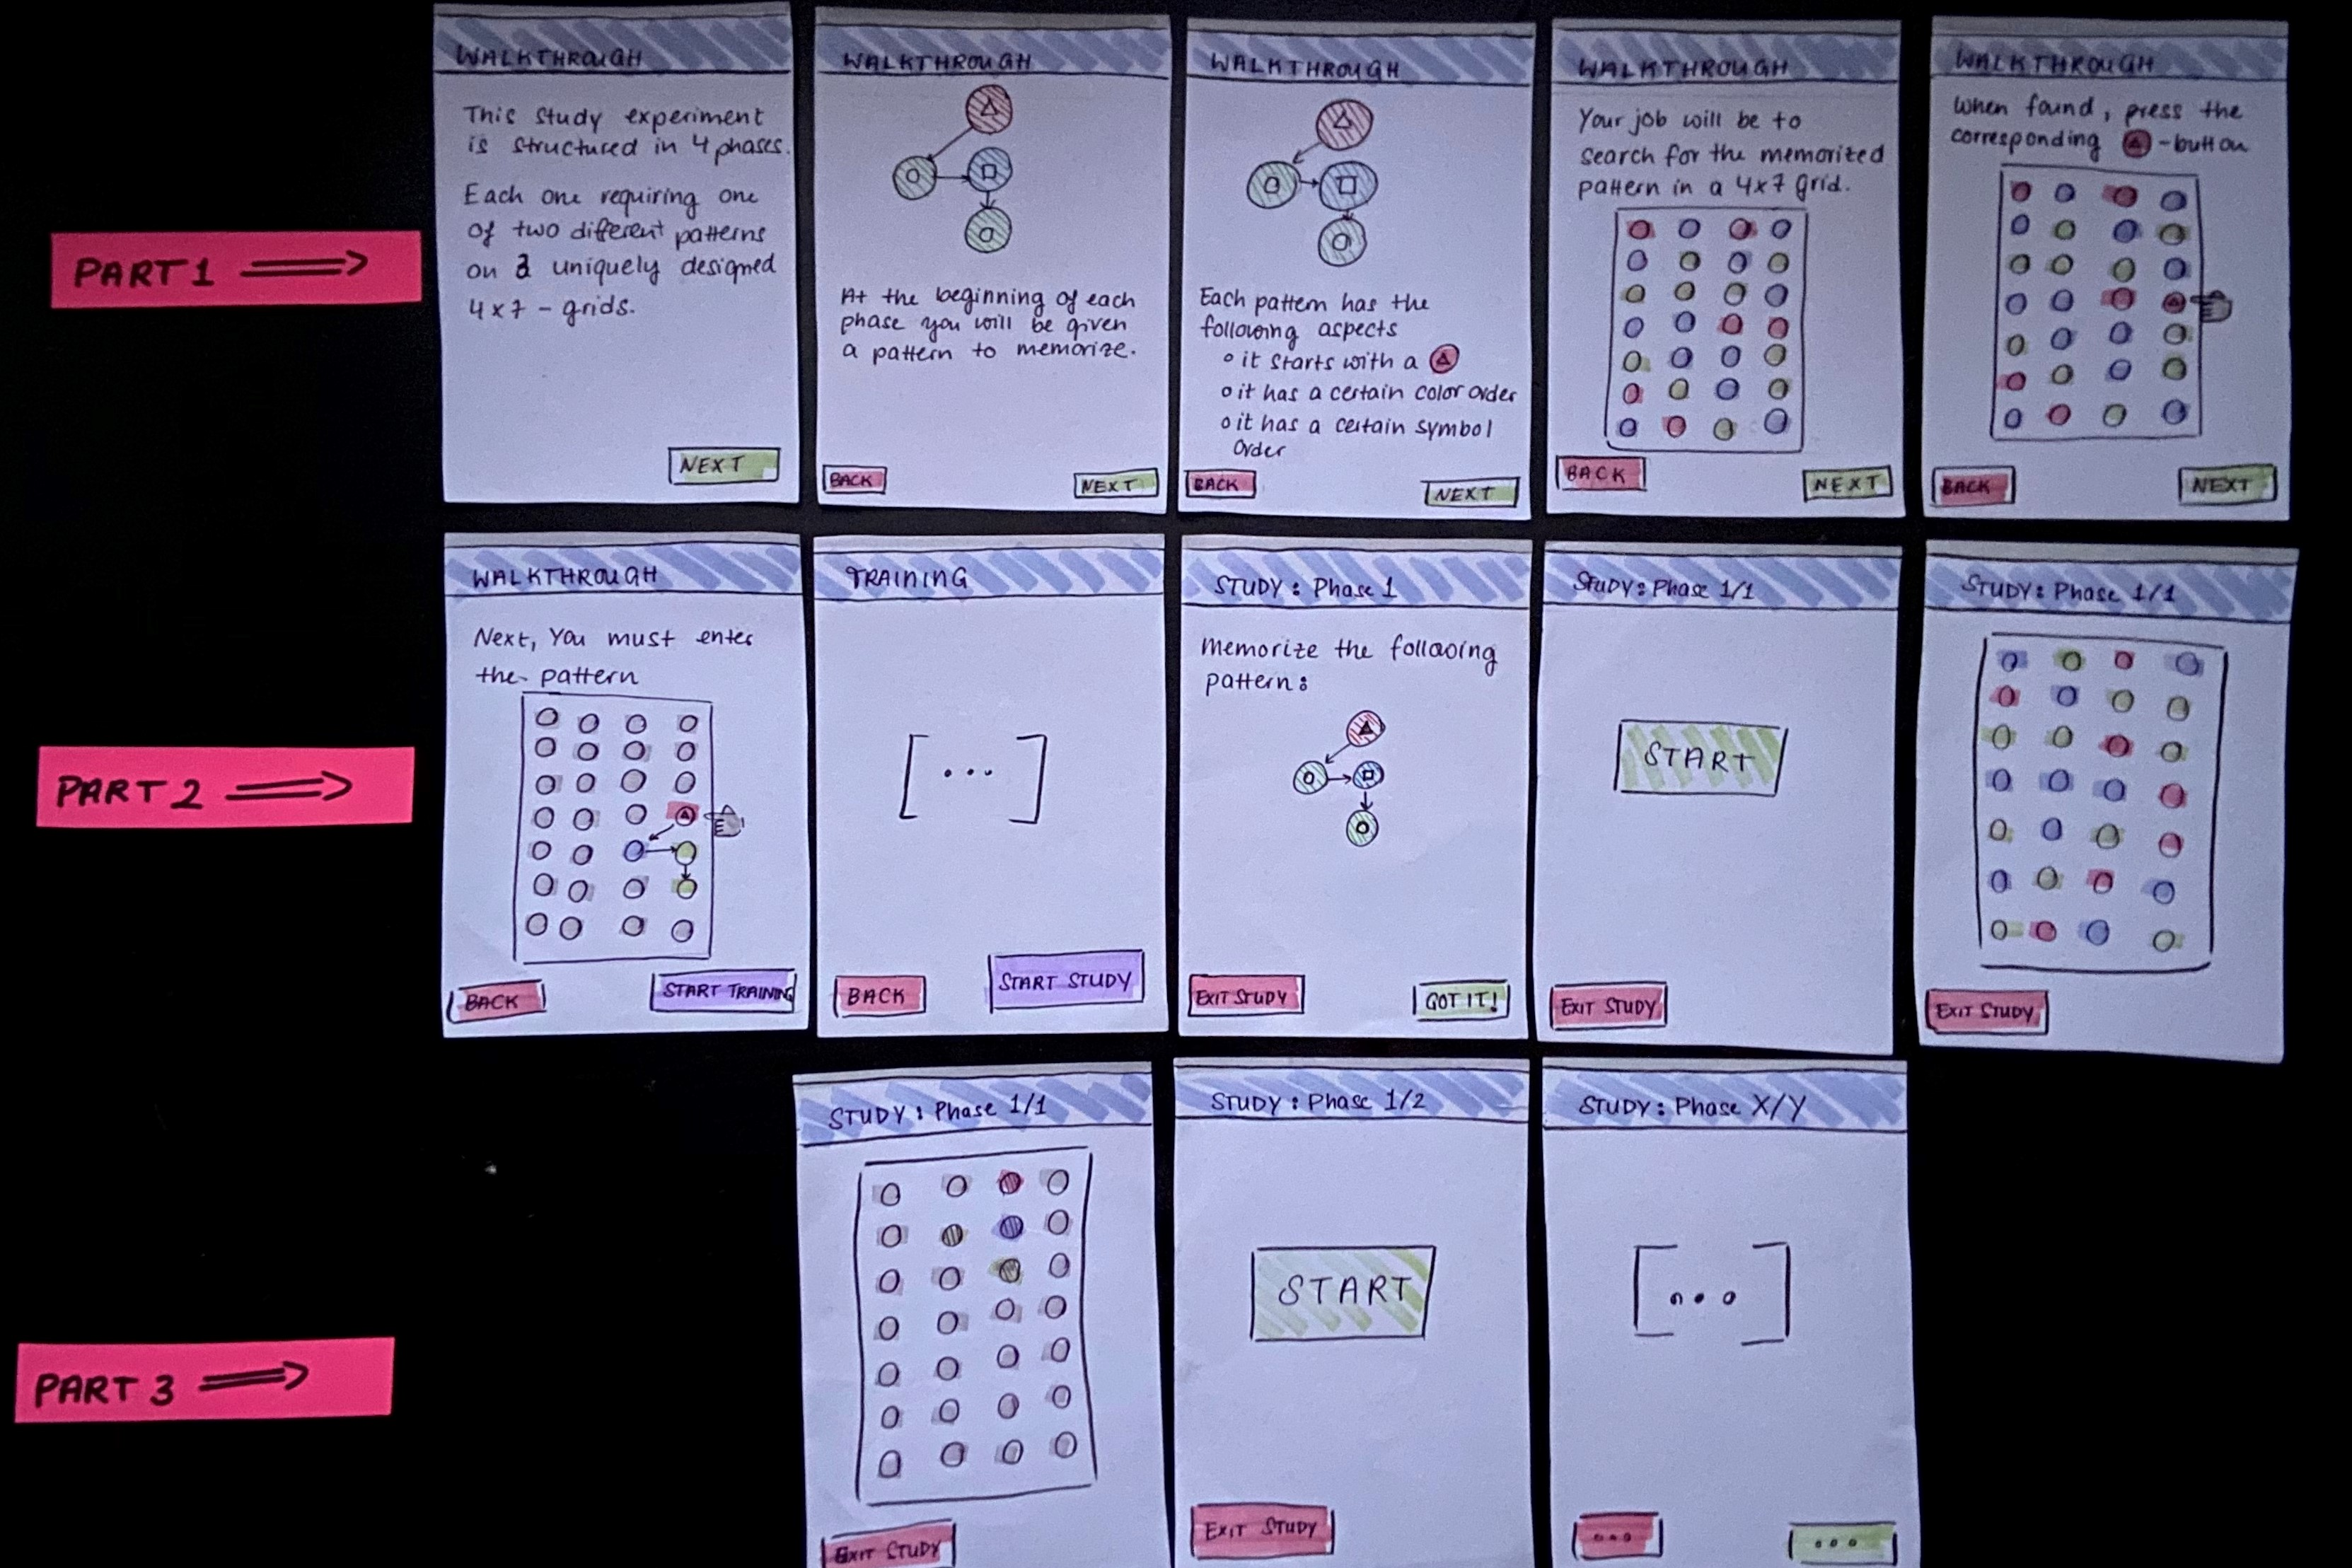
\includegraphics[width=15cm, height=15cm]{Chapters/graphics/pitch.jpg}
\caption{This picture illustrates the initial conception of the application's structure and flow. Although the developed application sightly differs from the cards, they served as a helpful base for the implementation of \underline{\textbf{FiPa}}.}
\label{fig:fipapitch}
\end{figure}
   
\section{Implementation} \label{4.3}

The following section presents the implementation of the concept \underline{\textbf{FiPa}}. I will begin by explaining the structure of the application and certain features which were embedded into it. As mentioned in the beginning of this chapter, \underline{\textbf{FiPa}} was solely intended to be a supportive tool to help us validate the findings made by Zezschwitz et al. \cite{Zezschwitz}, later in our complementary study (see Chapter \ref{ch:fifth}). For that, I will not deal with exact details of its framework, to avoid distraction from the fundamental purpose of this thesis.\\

\underline{\textbf{FiPa}} was implemented as an Android application, using the Software \textit{Android Studio}, which is based on IntelliJ IDEA. It is comprised of a series of classes, called activities. They can be seen as the fundamental building blocks of an application. Each activity describes and controls the functions of the user interface (UI) presented in a window on the screen\footnote{https://developer.android.com/guide/components/activities/intro-activities - last accessed: 2020/01/03.}. The structure of the UI is defined by a so-called layout, which is an XML-file that defines the features (i.e., images, buttons, strings) presented in a particular window\footnote{https://developer.android.com/guide/topics/ui/declaring-layout - last accessed: 2020/01/03.}. Activities within an application are able to communicate with each other and they determine the following event of each action inside a window. 


\subsection{Phase Structure} \label{4.3.1}

\begin{figure}[t!]
\centering
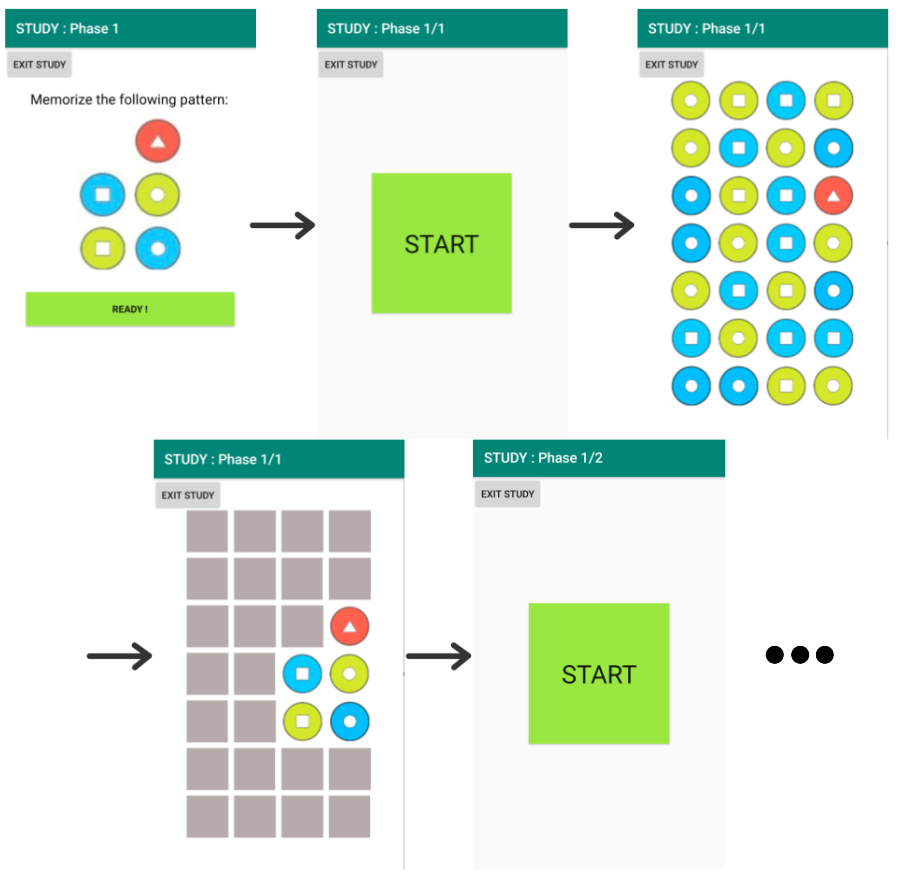
\includegraphics[width=15cm, height=14cm]{Chapters/graphics/phase.PNG}
\caption{This image illustrates the structure of a phase in the application. The remaining parts of the phase (Phase 1/2 and Phase 1/3) are analogious to the first part (Phase 1/1).}
\label{fig:appphase}
\end{figure}

The elemental structure of the application was first assessed by creating a simple illustration using cards (see Figure \ref{fig:fipapitch}). The intention behind this approach was to create a precise conception of the activity flow. Analogous to the design of our prototype (see Figure \ref{fig:paperprototype}), the application consisted of \underline{three distinct parts}. Each part represented a distinct ratio and was called  \textit{phase}\footnote{Not to confuse with Zezschwitz et al.'s interpretation of a phase, in Chapter \ref{ch:third}.}. 
Each \underline{phase} consisted of three \textbf{couples} (a combination of \textbf{mental} and \textbf{practical task}). In the application each \textbf{couple} was described as a \textit{level}, meaning each \textit{phase} consisted of three \textit{levels}. Similar to the paper prototype (see Figure \ref{fig:paperprototype}), each \textit{phase} also had a corresponding pattern assigned to it. As mentioned earlier in this chapter, one of my goals for the design of the concept was to minimize the amount of mental effort required for the interaction. For that, the ratios \textit{short orientation/short input} and \textit{long orientation/short input} shared the same short pattern. That way, participants only had to memorize two patterns, instead of three.\\

All \textit{phases} have the same flow. The first activity of each \textit{phase} shows an assigned pattern on the screen (see Figure \ref{fig:appphase}). The order in which the buttons should be entered, is conveyed through a simple animation. When the pattern is memorized, the user can proceed by pressing a green \textit{"READY"}-button. The next activity presents a layout with a green squared \textit{"START"}-button (see Figure \ref{fig:appphase}). This activity is of great importance as it defines the starting point of the \textbf{mental task}, meaning the beginning of the \textit{orientation phase}. The measurement of the \textit{orientation time} is initiated as soon as the \textit{"START"}-button is pressed and ends in the next activity, as soon as the user taps the correct \textit{starter-button} in the grid (see Figure \ref{fig:appphase}). This action causes a transformation: All buttons in the grid are blended out, except for the ones belonging to the pattern (see Figure \ref{fig:appphase}). The transformation is meant to convey to the user that they can execute the \textbf{practical task}, meaning the \textit{input phase}. The measurement of the \textit{input time} is initiated through the first button-press, given the correct \textit{starter-button} is selected, and ends when the last button of the pattern is pressed, given the pattern was entered correctly. If not, the time for \textit{input phase} cannot be stored in the database, and is marked as \textit{"failed"}. Analogous to the prototype, in Section \ref{4.2.2.4}, the \textit{starter-button} was meant to be pressed twice: Once to signify the find of the pattern and end the measurement of \textit{orientation time}, and once again to initiate the beginning of the \textit{input phase}. 

This process\footnote{Here we distinctively mean the process starting with the \textit{START}-button onward.} repeats itself for the following two levels of each phase. At the end of each phase the following phase automatically begins by presenting the next pattern.

\begin{figure}[t!]
\centering
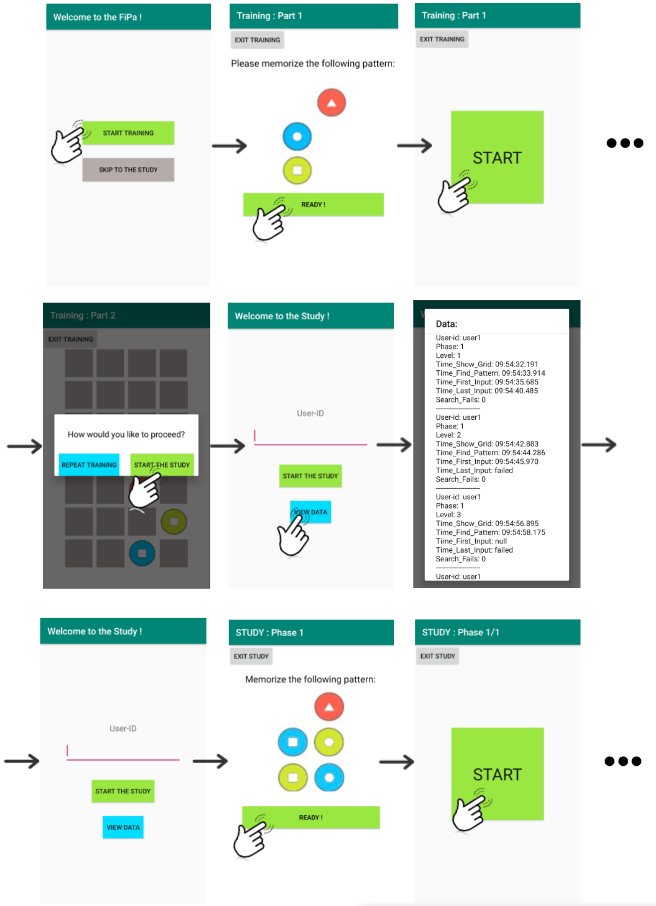
\includegraphics[width=15cm, height=21cm]{Chapters/graphics/flow.PNG}
\caption{This images is a rough representation of the application flow.}
\label{fig:flow}
\end{figure}

\subsection{Application Flow and Features} \label{4.3.2}

In the following section, we will present the flow of our application \underline{\textbf{FiPa}}, whilst introducing its special features along the way. \\

The first activity of the application presents window which allows the user to choose whether they would like to proceed with the training-segment or skip to the study (see Figure \ref{fig:flow}). Assume we were to proceed with the training. The training segment presents an exercise walk-through of the concept, meant to get the user acquainted with the concept of \underline{\textbf{FiPa}} and to minimize the amount of errors made throughout the study. At the end of the training-segment, users have the option to proceed with the study or repeat the training (see Figure \ref{fig:flow}). It was important to assure that participants truly understood the functioning of the concept. For that they able to repeat the training-segment as often as they felt necessary. Assume we were to proceed with the study. The next activity is responsible for the maintenance of the collected data. It allows to enter a user-id for the user, which helped to pair a user's collected quantitative data (measurements) with their qualitative data (survey answers) later in evaluation (see Figure \ref{fig:flow}). Moreover, it was possible to view the content of the local database through the application (see Figure \ref{fig:flow}). This feature was useful during the development of the application, to assure that the phases (\textit{orientation} and \textit{input}) were measured correctly, and also in many cases during the study. From this point, let us assume we were to start the study (see Figure \ref{fig:flow}). This action would lead us to the first phase of the concept. As described in Section \ref{4.3.2}, each phase begins by presenting its corresponding pattern, intended for memorization (see Figure \ref{fig:flow}). When the pattern is memorized, the user can proceed by pressing the \textit{"READY"}-button. It is important to note that buttons, used to approve or proceed, were intentionally given the color green, as it is it is commonly associated with the action "GO" or the approval "OK" in everyday life.\\

\begin{figure}[t!]
\centering
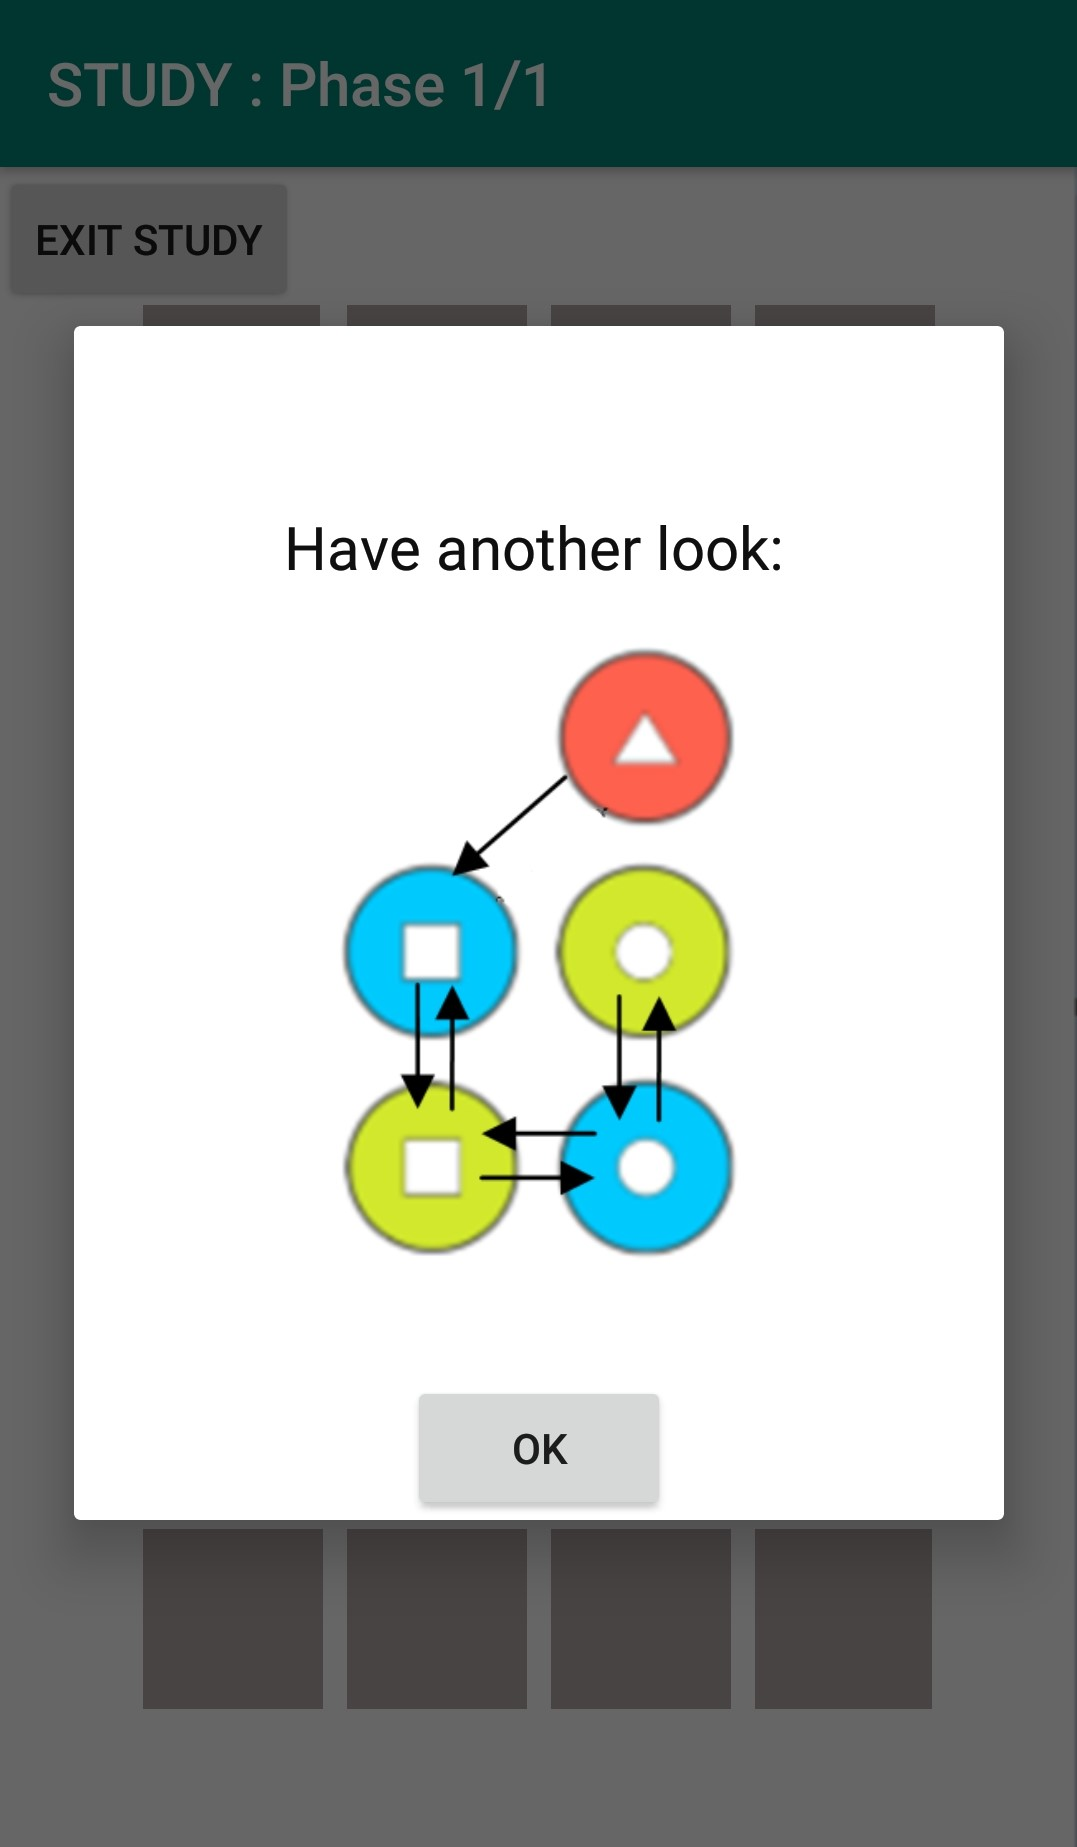
\includegraphics[width=6cm, height=9cm]{Chapters/graphics/error.jpg}
\caption{The \textit{error-recovery} of the application of implemented as a pop-up window which appeared when three errors were made. The pop-up was the same for search and input errors.}
\label{fig:errorpopup}
\end{figure}

Assume we were to proceed and begin with the Level 1 of Phase 1 (see Figure \ref{fig:flow}). At this point, we have to complete the \textbf{mental task}, which is to find the hidden pattern inside the grid. During the search process, the \textit{orientation time} is being measured in the background. The measurement is unnoticeable to the user during the interaction. As it is possible to press the wrong starter-button during the search process, we added a feature into the application which served as a form of \textit{error-recovery} (see Chapter \ref{ch:third}). It was realized through a pop-up window which appeared after the third search error was made (see Figure \ref{fig:errorpopup}). The pop-up illustrated the pattern to remind the user, in case they had forgotten it. As soon as the user found the pattern, the grid transformed as described in Section \ref{4.3.1} (see Figure \ref{fig:appphase}), signifying the beginning of the \textbf{practical task}. As errors were also possible during the input, we also included \textit{error-recovery} (see Figure \ref{fig:errorpopup}). Here, the pop-up window appeared after the third input error. After it appeared, the app proceeded with the next action and marked the input of the particular level as \textit{"failed"}. Although the main focus is to examine the effects of \textit{orientation time} and \textit{input time}, we could not avoid including an \textit{error-recovery phase}, as it would have negatively impacted the user-friendliness of the application\footnote{To assure that the \textit{error-recovery phase} did not have an impact on the results of our study, we took specific measures, which will be presented in Chapter \ref{ch:sixth}.}. The procedure of the two follow-up levels of the phase have the same presented procedure. The flow of the two following phases is analogous to the procedure presented in Section \ref{4.3.1} (see Figure \ref{fig:appphase}).  \\





